\section{A stronger simulation from the consistency graph}
\label{sec:consistency-graph}

Fixing every shared vertex is sufficient, but it discards the arrangement
of those vertices. The graph may permit a sequence of small intermediate
tables even when the total number of shared values is large. We now use
that arrangement. The proof combines a circuit-specific count of consistency
constraints with a published theorem on pathwidth. Its quantitative
consequence improves the preceding $1/3$ exponential rate to $1/5$.

The basic operation is simple: keep a table of which assignments to the
current boundary can be extended through the processed part. Each table
entry is a circuit on $x$. Ordinary inputs remain shared circuit wires;
they are never enumerated as table indices.

\subsection{Separate ordinary computation from consistency}

Normalize and prune the supplied circuit. If its output has no syntactic
witness dependency, its existing circuit computes the projection. If its
output is a witness input, the projection is one. Otherwise partition the
gates into $p$ gates independent of the witnesses and $q\ge1$ dependent
gates. Compute the independent gates once. Let
$h_1(x),\ldots,h_h(x)$ be the distinct independent signals entering
dependent gates, including direct ordinary inputs, and let $b$ be the
number of used witnesses. Let $\ell$ count input pins of dependent
gates supplied by a witness or a dependent gate. Then
\begin{equation}\label{eq:core-pins}
 \ell+h\le2q.
\end{equation}
Here $h$ counts distinct signals, while $\ell$ counts pins, with
multiplicity. Every dependent gate has at least one dependent input,
so it has at most one independent input.

Introduce a consistency variable for every witness and every dependent
gate output. A gate $v$ contributes the constraint
\[
 A_v=[z_v=\operatorname{op}_v(\text{predecessor values})],
\]
and the output contributes $[z_{\mathrm{out}}=1]$. The ordinary
signals in these expressions remain functions of $x$. Form a bipartite
incidence graph $H$ with one vertex for each consistency variable and
each constraint, and one edge for each incidence. Retain multiple
incidences if a value supplies two pins.

\begin{lemma}[The consistency budget]\label{lem:consistency-budget}
The graph $H$ is connected and has
\[
 |V(H)|=2q+b+1,\qquad |E(H)|=q+\ell+1.
\]
Its cycle rank $\kappa=|E(H)|-|V(H)|+1$ therefore satisfies
\begin{equation}\label{eq:consistency-budget}
 \boxed{\quad \kappa=\ell-q-b+1,\qquad h+b+\kappa\le q+1.\quad}
\end{equation}
If the full cone has $s=p+q$ gates and $a$ used ordinary inputs, then
also $\kappa\le s+1-a-b$.
\end{lemma}
\begin{proof}
Every dependent gate and used witness has a directed path through
dependent gates to the output. The incidence graph subdivides those
connections and adds the output constraint, proving connectivity and
the counts. Equation~\eqref{eq:core-pins} gives the boxed inequality.
For the last assertion, delete the ordinary inputs and independent
gates from the full cone's underlying undirected multigraph. The
remaining graph has $q+b$ vertices and $\ell$ edges, and hence cycle
rank $\kappa$. Deletion cannot increase cycle rank, as follows by
restricting the binary cycle space. The full cone has at most $2s$
edges and $s+a+b$ vertices, giving the claimed bound.
\end{proof}

The conjunction of the constraints, quantified over all consistency
variables, equals $g$. An original witness assignment extends uniquely
to its gate values. Conversely, the equations force those values by
topological induction. This observation preserves the consistency that
naive separate existential evaluation loses.

\subsection{Small tables reduce the graph to a cubic graph}

Give every incidence edge its own binary index. At a variable vertex,
place the equality table: its entry is one exactly when all incident
indices agree. At a constraint vertex, place the constraint's truth
table on its incident indices. A degree-one equality table has both
entries one. A gate table has at most three indices. After fixing its
indices, its entry is a constant, some $h_i(x)$, or its complement.
Thus the $p$ independent gates and at most $h$ additional complements
prepare every table entry.

We call these arrays \emph{Boolean tensors}; no numerical approximation
is involved. Contracting an edge means ORing over its binary value and
ANDing the two incident entries. Distributivity proves that contraction
preserves the represented function, pointwise for each fixed $x$.

\begin{lemma}[A cubic reduction with linear circuit cost]
\label{lem:cubic-reduction}
The consistency tables reduce, using $O(q+1)$ extra gates, to a scalar
factor and either an empty graph or a simple connected cubic graph
$K$. If $N=|V(K)|>0$, then
\[
 N=2(\kappa(K)-1)\le2(\kappa-1).
\]
Every surviving table still has at most eight entries, each represented
by an already constructed circuit wire.
\end{lemma}
\begin{proof}
First replace each equality vertex of degree $D\ge4$ by a tree of
$D-2$ ternary equality vertices. The internal edge values are uniquely
determined when the external values agree. This adds $D-3$ vertices
and edges, preserving cycle rank and connectivity. The new equality
vertex count is at most the sum $q+\ell+1$ of the old variable degrees.
Including constraint vertices, the resulting subcubic graph has
\[
 N_0\le q+1+(q+\ell+1)\le4q+2
\]
vertices. A loop counts twice toward degree.

Apply the following exact table operations until none applies.
\begin{enumerate}
 \item Remove a rank-zero table and AND its scalar into an accumulator.
 \item For a loop, identify its two ports and OR the two diagonal
 entries. There are at most two remaining entries. Summing all four
 combinations would violate the equality of the loop's two ends.
 \item At a loop-free vertex of degree one or two, contract one edge
 into its neighbor. The resulting rank is at most three. Each of at
 most eight entries needs two ANDs and one OR, costing at most 24 gates.
 Any second edge between the same vertices becomes a loop.
 \item If two cubic vertices share two edges, contract both at once.
 The four resulting entries each use four ANDs and three ORs, costing
 28 gates. Three parallel edges instead produce one scalar using at
 most 15 gates.
\end{enumerate}
Each operation decreases $|V|+|E|$, costs at most 32 gates, and keeps
degree at most three. Initially $|E|\le3N_0/2$, so 80$N_0$ gates
suffice for all reductions, including the scalar accumulator.

Contracting an ordinary edge preserves cycle rank; removing a loop
lowers it by one; contracting $j$ parallel edges lowers it by $j-1$.
The remaining nonempty graph stays connected. At termination it is
simple and every degree is three. Hence $|E(K)|=3N/2$, and its cycle
rank is $N/2+1$. This proves the assertion.
\end{proof}

The treatment of loops and parallel edges matters. Silently deleting
them as graph-theoretic nuisances would change the represented function.
The reductions above manipulate their actual tables at a charged cost.

\subsection{From a path decomposition to a circuit}

A \emph{path decomposition} is a sequence of bags containing all
vertices, containing both ends of every edge in some bag, and containing
each vertex in a consecutive interval of bags. Its width is the largest
bag size minus one; pathwidth is the minimum such width. The cutwidth
of a vertex ordering is the largest number of edges crossing between
a prefix and the remaining vertices.

\begin{lemma}[A width conversion for cubic graphs]\label{lem:median-width}
A simple cubic graph of pathwidth $k$ has a vertex ordering of cutwidth
at most $k+2$.
\end{lemma}
\begin{proof}
Given bags $B_1,\ldots,B_L$, represent $v$ by
$I_v=[\operatorname{first}(v)-1/4,\operatorname{last}(v)+1/4]$.
At most $k+1$ intervals contain any point. For each edge $e=uv$ choose
a distinct timestamp $t_e$ in the interior of $I_u\cap I_v$, which
is nonempty. Place $v$ at the median $t_v$ of its three incident
timestamps and order the vertices by these medians.

Consider a cut at a point $t$ distinct from all timestamps. For a
crossing edge with $t_u<t<t_v$, charge it to $u$ if $t_e>t$, and to
$v$ otherwise. The charged interval contains $t$. A vertex receives
at most one charge: it has just one incident timestamp strictly above
its median and just one strictly below it. Thus there are at most
$k+1$ crossing edges.

At a cut between tied medians, at most two vertices are tied, because
the edge timestamps are distinct and an edge has two endpoints. Apply
the same charging rule to every other crossing edge. Only the edge
whose timestamp equals the common median can remain uncharged, adding
at most one. This proves the $k+2$ bound and gives an explicit ordering.
\end{proof}

This width conversion is consistent with established graph-search
relations; it is included with a proof to make the numerical exponent
checkable. Section~\ref{sec:prior-work} records the attribution.

\begin{lemma}[Symbolic frontier contraction]\label{lem:frontier}
Given an ordering of $K$ of cutwidth $w$, its tensor value has a circuit
using fewer than $4N2^w$ additional gates.
\end{lemma}
\begin{proof}
Let $F_i$ be the edges leaving the first $i$ vertices. For each
$\alpha\in\B^{F_i}$ maintain a wire $P_i(\alpha;x)$: the OR over
internal edge assignments of the AND of all processed table entries,
with the boundary fixed to $\alpha$. Start with $P_0=1$.

At the next vertex let $J$ be its $j$ edges into the processed prefix.
For each new boundary assignment, OR over the $2^j$ assignments to
$J$ the AND of the appropriate old entry and local table entry. This
preserves the stated meaning by distributivity. Its gate cost is
\[
 2^{|F_i|}(2^{j+1}-1)<2^{|F_i|+j+1}.
\]
Because $|F_i|=|F_{i-1}|+3-2j$ and both frontier sizes are at most
$w$, one has $|F_i|+j\le w+1$: use the new frontier for $j=0,1$
and the old frontier for $j=2,3$. Each vertex therefore costs less
than $2^{w+2}$ gates. At the last vertex there are no boundary indices
and the single entry is the desired scalar.
\end{proof}

The complete finite construction costs at most
\begin{equation}\label{eq:finite-tensor-cost}
 p+h+80N_0+4N2^w+1\le p+400(q+1)2^w.
\end{equation}
For an empty reduced graph the frontier construction is unnecessary;
take $N=w=0$ and use the scalar accumulator. Ordinary computation is
paid once, including when its result appears in many boundary entries.

\subsection{The improved exponential rate}

We use the following published graph theorem: for every $\eta>0$
there is $n_\eta$ such that every simple subcubic graph on $N>n_\eta$
vertices has pathwidth at most $(1/6+\eta)N$. A suitable decomposition
can be constructed in polynomial time for fixed $\eta$
\citep[Theorem 5 and Section 4]{FominHoie2006}.

\begin{theorem}[Projection controlled by consistency cycles]
\label{thm:cycle-simulation}
For every $\delta>0$ there is a constant $A_\delta$ such that
\begin{equation}\label{eq:cycle-simulation}
 \C(g)\le p+A_\delta(q+1)2^{(1/3+\delta)\kappa}.
\end{equation}
For example, $A_\delta=400\cdot2^{n_{\delta/2}+2}$ suffices using
the threshold in the cited theorem. No uniform small value of this
constant, or endpoint bound $O((q+1)2^{\kappa/3})$, is asserted.
\end{theorem}
\begin{proof}
Use the cubic reduction and the graph theorem with $\eta=\delta/2$.
Since $N\le2\kappa$, Lemma~\ref{lem:median-width} gives
$w\le(1/3+\delta)\kappa+2$ for large $N$. The finitely many smaller
graphs are covered by adding $n_{\delta/2}$ to the exponent. Apply
\eqref{eq:finite-tensor-cost}.
\end{proof}

\begin{theorem}[A universal $1/5$ exponential rate]\label{thm:fifth}
Set $\alpha=1/3+\delta$ and $\beta=\alpha/(1+2\alpha)$.
With the preceding notation,
\begin{equation}\label{eq:core-fifth}
 \C(g)\le p+O_\delta\!\left((q+1)
                    2^{\min\{h,b,\alpha\kappa\}}\right)
 \le p+O_\delta\!\left((q+1)2^{\beta(q+1)}\right).
\end{equation}
In particular, for every $\varepsilon>0$,
\begin{equation}\label{eq:fifth}
 \boxed{\quad
 D(n,m,s)=O_\varepsilon\!\left(
  \min\left\{\frac{2^n}{n},\ (s+1)2^m,
       (s+1)2^{(1/5+\varepsilon)(s+1)}\right\}\right).
 \quad}
\end{equation}
The comparison with $2^n/n$ assumes $n\ge2$ as before.
\end{theorem}
\begin{proof}
Two alternatives to \eqref{eq:cycle-simulation} are
$p+O((q+1)2^b)$ by witness enumeration and $p+M_h$ by treating
the $h$ independent signals as formal input bits. Substituting their
actual values after synthesis is valid even when those values are
correlated. The bound $M_h=O(2^h)$, also valid for $h=0,1$, suffices.
Take the minimum of these three estimates. If
$z=\min\{h,b,\alpha\kappa\}$, the consistency budget gives
\[
 (2+1/\alpha)z\le h+b+\kappa\le q+1.
\]
This proves \eqref{eq:core-fifth}. Since $\beta\to1/5$ as
$\delta\downarrow0$, and $p+q\le s$ after normalization, the
claimed universal bound follows. Trivial outputs were handled before
the construction.
\end{proof}

This is a circuit-size theorem. In particular, the synthesis of an
arbitrary function on the formal inputs does not promise that its
truth table can be discovered in the size of the resulting circuit.
The numerical rate comes from three precise facts: $h+b+\kappa\le q+1$,
at most $2\kappa$ vertices in the cubic reduction, and pathwidth at
most $N/6+o(N)$. It is not a claim that the coefficient $1/5$ is optimal.

\begin{figure}[ht]
\centering
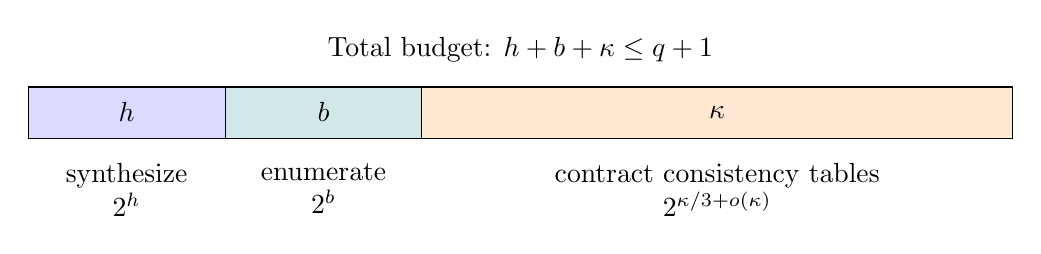
\begin{tikzpicture}[x=1.25cm,y=1cm]
 \fill[blue!14] (0,0) rectangle (2,0.65);
 \fill[teal!18] (2,0) rectangle (4,0.65);
 \fill[orange!18] (4,0) rectangle (10,0.65);
 \draw (0,0) rectangle (10,0.65);
 \draw (2,0)--(2,0.65) (4,0)--(4,0.65);
 \node at (1,0.33) {$h$};
 \node at (3,0.33) {$b$};
 \node at (7,0.33) {$\kappa$};
 \node[anchor=south] at (5,0.85) {Total budget: $h+b+\kappa\le q+1$};
 \node[align=center,anchor=north] at (1,-0.2)
   {synthesize\\$2^h$};
 \node[align=center,anchor=north] at (3,-0.2)
   {enumerate\\$2^b$};
 \node[align=center,anchor=north] at (7,-0.2)
   {contract consistency tables\\$2^{\kappa/3+o(\kappa)}$};
\end{tikzpicture}
\caption{The limiting balance is $h:b:\kappa=1:1:3$.
All three exponents then approach $(q+1)/5$.
This balances upper bounds; it supplies neither a hard example nor
a proof that this rate is optimal. Ordinary preprocessing costs $p$
additional gates, once.}
\label{fig:consistency-budget}
\end{figure}

\paragraph{Why the independent part should stay outside the exponent.}
For $t\ge3$, put $a_i=x_{2i-1}\land x_{2i}$ and
\[
 H_t(x)=\bigoplus_{1\le i<j\le t}(a_i\land a_j),
 \qquad f_t(x,y)=H_t(x)\land(y_1\lor\cdots\lor y_t).
\]
Compute all $a_i$, their pair products, an XOR chain, the witness OR
chain, and the final AND. This supplied circuit has
$p=t^2-1$, $q=b=t$, $h=1$, and $\kappa=0$.
The projection is $H_t$, with a circuit of size $p$.
Every ordinary input is essential: set one other $a_j$ to one,
all remaining pairs to zero, and the other bit of the chosen pair to
one. Every witness is essential when $H_t=1$ and the other witnesses
are zero. Thus unused inputs do not explain the simplification.

The full undirected circuit graph contains a subdivision of $K_t$,
with the $a_i$ as branch vertices and their pair-product gates on
the edges. Its treewidth is at least $t-1$, although the consistency
graph is a tree. Also $r=t$ for the old shared-vertex bound, whereas
the new structural bound is $O(t^2)$. Coverage independently detects
a one-witness cover in this example. The example explains a distinction
between structural parameters, not a circuit lower bound or an example
attaining the $1/5$ exponent.

\subsection{Condition a few values before eliminating the rest}

\begin{corollary}[Conditioning and componentwise elimination]
\label{cor:condition-cycles}
Fix $t$ consistency variables in every possible way, retaining all
defining equations. Let $\kappa_*$ be the largest cycle rank of a
connected component of the remaining incidence graph. Then
\[
 \C(g)\le p+O_\delta\!\left((q+1)
                  2^{t+(1/3+\delta)\kappa_*}\right).
\]
\end{corollary}
\begin{proof}
In each branch, distinct components have disjoint quantified variables.
Their projections may therefore be ANDed for each fixed $x$. Apply the
construction to each component; their total size is $O(q+1)$ and their
individual exponents are bounded by $(1/3+\delta)\kappa_*$. OR the
$2^t$ branches. The independent signals remain shared. Consistency
equations make the conditioning sound, exactly as in Theorem~\ref{thm:cut}.
\end{proof}

Conditioning combined with elimination is an established algorithmic
architecture. Here it supplies a refinement of the explicit circuit
bound, useful when a small set of shared values separates otherwise
difficult parts. The relevant exponent uses the largest residual
component, rather than the sum of its components' cycle ranks.

\subsection{The uniform SAT and exact-counting algorithm}
\label{sec:counting-algorithm}

We now prove the algorithmic guarantee highlighted in
Section~\ref{sec:algorithm-overview}. The nonuniform theorem used
synthesis on formal ordinary inputs.
The all-quantified case has no such step. Its explicit table operations
also preserve counts, which gives the following algorithmic consequence.
This statement includes its proof; the unresolved issue in
Section~\ref{sec:prior-work} is comparison and priority.

\begin{corollary}[Counting by the gate-minus-input budget]
\label{cor:gate-counting}
Fix $\delta>0$ and write $\alpha=1/3+\delta$. Given a single-output
$B_2$ circuit with $s$ gates and $u$ input bits, one can count its
satisfying inputs in time
\[
 \poly_\delta(s+u+1)\,
 2^{\min\{b,\alpha(s+1-b)\}},
\]
where $b$ is the number of inputs remaining in a normalized output
cone. In particular, for every fixed $\varepsilon>0$, the time is
\[
 \poly_\varepsilon(s+u+1)\,
 2^{(1/4+\varepsilon)(s+1)}.
\]
The space used is at most polynomial times the same exponential
factor. A polynomial-space bound is not asserted.
\end{corollary}
\begin{proof}
Prune the output cone and propagate constants and unary redundancies
without changing the function. Inputs removed from the cone are free;
their contribution is a final multiplicative factor $2^{u-b}$.
Constant and designated-input outputs are evaluated directly. For the
remaining circuit quantify all $b$ inputs, so there are no independent
signals. Its consistency rank satisfies $\kappa\le s+1-b$.

Replace Boolean OR and AND in the tensor construction by integer
addition and multiplication. The original tables contain only zeros
and ones. For each satisfying input, the circuit equations specify
exactly one gate-value assignment. Incidence equality tables specify
exactly one set of equal edge values, and their ternary expansions have
exactly one internal extension. Thus the initial tensor contraction
counts satisfying inputs, with no spurious multiplicity.

Every reduction in Lemma~\ref{lem:cubic-reduction} is a distributive
identity, including diagonal loop sums and joint parallel-edge sums.
It remains valid over the nonnegative integers. More explicitly, a
reduced table entry is the number of internal edge assignments in its
contracted region that satisfy the original tables, conditional on its
boundary. A contraction combines disjoint regions and sums over their
shared indices, preserving this interpretation. The same invariant
holds for the frontier entries in Lemma~\ref{lem:frontier}.

There are $O(s+1)$ indices after equality expansion. Each table entry
is therefore bounded by $2^{O(s+1)}$, so its bit length is $O(s+1)$.
Integer additions and multiplications have polynomial bit cost; the
last factor $2^{u-b}$ only shifts the answer. For fixed $\delta$, the
cited constructive pathwidth theorem and median conversion find the
required order in polynomial time. The bounded-size graphs below its
threshold are handled by exhaustive order search, a constant depending
on $\delta$. The operation count is consequently polynomial times
$2^{\alpha(s+1-b)}$, with exponential-size frontiers allowed.

Alternatively enumerate the $2^b$ used-input assignments, evaluate the
circuit, and count the accepting ones. Choose the cheaper proved bound.
Finally,
\[
 \min\{b,\alpha(s+1-b)\}
 \le\frac{\alpha}{1+\alpha}(s+1),
 \qquad \frac{\alpha}{1+\alpha}\longrightarrow\frac14.
\]
This proves both time estimates and the stated space majorant.
\end{proof}

Testing whether the count is nonzero decides circuit satisfiability.
For any fixed $0<\gamma<4$, the bound also gives a running time
$2^{(1-\Omega_\gamma(1))u}\poly(u)$ when
$s\le(4-\gamma)u$, after choosing a sufficiently small fixed
$\varepsilon$. This consequence uses exponential space and the exact
$B_2$ gate convention. Its numerical comparison with previously
reported circuit-SAT algorithms deserves particular scrutiny.

\subsection{What critical amplification would force}
\label{sec:critical-balance}

The coefficient $1/5$ comes from balancing three upper bounds.
Near equality therefore forces several structural conditions
simultaneously. The following statements concern a normalized circuit
with $q\ge1$ and a witness-dependent gate as output, using the notation
of Section~\ref{sec:consistency-graph}.

\begin{lemma}[Finite stability of the three-way balance]
\label{lem:finite-stability}
Fix $\delta>0$, put $\alpha=1/3+\delta$, and choose $A_\delta\ge1$
large enough for
\[
 \C(g)\le p+A_\delta(q+1)2^{\min\{h,b,\alpha\kappa\}}.
\]
If $t\ge0$ and $\C(g)\ge p+A_\delta(q+1)2^t$, then
\[
 \Delta=q+1-(2+1/\alpha)t\ge0,
\]
and there are $e_h,e_b,e_\kappa\ge0$ satisfying
\[
 h=t+e_h,\qquad b=t+e_b,\qquad
 \kappa=t/\alpha+e_\kappa,\qquad
 e_h+e_b+e_\kappa\le\Delta.
\]
\end{lemma}
\begin{proof}
Comparing the two size inequalities forces
$h,b,\alpha\kappa\ge t$. Subtract these lower bounds from
$h+b+\kappa\le q+1$.
\end{proof}

This elementary lemma is useful because it preserves the fixed-$\delta$
constant before any limit is taken. Its asymptotic consequence also
constrains the residual graph, beyond the original cycle count.

\begin{theorem}[Necessary structure at the critical gate budget]
\label{thm:critical-structure}
Consider a family with $m\to\infty$ declared witness bits, normalized
size $s=p+q$, and
\[
 s+1=(5+o(1))m,\qquad \log\C(g)\ge m-o(m).
\]
Let $a$ be the number of used ordinary inputs. Then
\begin{align*}
 p&=o(m),& q&=(5+o(1))m,\\
 a,h,b&=(1+o(1))m,& \kappa&=(3+o(1))m.
\end{align*}
For every choice of legal equality splitting and reductions in
Lemma~\ref{lem:cubic-reduction}, the resulting kernel $K$ is
eventually nonempty and satisfies
\begin{align*}
 |V(K)|&=(6+o(1))m,& \kappa-\kappa(K)&=o(m),\\
 \operatorname{cw}(K)&=(1+o(1))m,&
 \operatorname{pw}(K)&=(1+o(1))m.
\end{align*}
Here cutwidth and pathwidth mean their minimum over all orders and
decompositions. No hard family satisfying the hypotheses is asserted.
\end{theorem}
\begin{proof}
Since $p=O(m)$ whereas $\C(g)\ge2^{m-o(m)}$,
$\log(\C(g)-p)\ge m-o(m)$. For each fixed $\delta>0$,
Theorem~\ref{thm:fifth} therefore gives
\[
 h\ge m-o(m),\qquad b\ge m-o(m),\qquad
 \kappa\ge m/\alpha-o(m).
\]
The prefactor contributes only $O_\delta(\log m)$ to the logarithm.
Using $p+h+b+\kappa\le s+1$, we obtain
\[
 \limsup \frac{p}{m}\le3-1/\alpha,\qquad
 \limsup \frac{h}{m},\ \limsup\frac{b}{m}\le4-1/\alpha.
\]
These inequalities hold for every fixed $\delta$. Letting $\delta$
tend to zero after taking the limits proves $p=o(m)$ and
$h/m,b/m\to1$. The budget and the fixed-$\delta$ lower bounds
then give $\kappa/m\to3$, and $q/m\to5$ follows from $s=p+q$.

To relate $a$ to $h$, note first that $h\le a+p$. In the undirected
graph on the $a$ ordinary inputs and $p$ independent gates, every
connected component contains an interface signal, because every
vertex is in the output cone. If there are $c$ components, then
$c\le h$, and counting edges gives
$a+p-c\le2p$. Thus $a\le p+h$, so $|a-h|\le p$ and $a/m\to1$.

Fix any sequence of legal reductions along the family. An empty
kernel would give $\C(g)=O(s)$, so eventually it is nonempty.
Write $N=|V(K)|$. The finite compiler bound, applied to an order
of minimum cutwidth, gives
\[
 \C(g)\le p+400(q+1)2^{\operatorname{cw}(K)},
 \qquad \operatorname{cw}(K)\ge m-o(m).
\]
The cutwidth lower bound and $\operatorname{cw}(K)\le3N/2$ imply
$N\to\infty$. On the other hand $N\le2(\kappa-1)\le6m+o(m)$. For every fixed
$\eta>0$, the cubic pathwidth theorem and
Lemma~\ref{lem:median-width} give, for sufficiently large $N$,
\[
 \operatorname{cw}(K)\le\operatorname{pw}(K)+2
       \le(1/6+\eta)N+2.
\]
Hence $\liminf N/m\ge1/(1/6+\eta)$ for every $\eta>0$, proving
$N/m\to6$. The cubic identity $\kappa(K)=N/2+1$ gives the cycle
loss. The same inequalities sandwich each width between $m-o(m)$
and $m+o(m)$. All constants depend only on the fixed slack, so this
argument applies to any selected legal reduction sequence.
\end{proof}

There is little unused fanin capacity in such a family. If $r$ counts
independent-signal input pins of the dependent gates, with multiplicity,
and $U=2q-(\ell+r)$, then
\[
 q+1-h-b-\kappa=U+(r-h)=o(m).
\]
Both terms are nonnegative. Thus only $o(m)$ input slots are missing
from binary gates, and ordinary signals have only $o(m)$ repeated
uses at the interface. This concerns distinct signals, not semantic
independence of their values.

\paragraph{Combining the structural and witness conditions.}
The hypotheses hold whenever $s+1=(5+o(1))m$ and
$\C(g)\ge T=2^m(s+1)/L$ with $\log L=o(m)$.
Corollary~\ref{cor:sparse-population} then also forces
$\Omega((T/n)\log(2+T/n))$ positive ordinary inputs with $O(nL)$
declared witnesses. Removing the $m-b$ unused witness bits divides
each positive fiber and this threshold by exactly $2^{m-b}$;
the two witness conventions must be kept consistent.
Enumeration already gives $m-b\le\log L$ under this amplification
hypothesis. These are simultaneous necessary conditions. Large
width, balanced budgets, and sparse fibers alone do not establish
a lower bound on $\C(g)$.

\subsection{Critical graph budgets can coexist with an easy projection}
\label{sec:kernel-realization}

The critical gate and cycle budgets alone do not force a hard
projection. A large class of cubic graphs can occur as exact residual
kernels with nearly critical budgets and a simple projection. The
distinction between the supplied circuit and a minimum circuit is
essential here.

\begin{theorem}[Cubic realization with controlled budgets]
\label{thm:kernel-realization}
Let $K$ be a finite simple 2-vertex-connected cubic graph and put
$k=|V(K)|/2+1$. Set $t=\lfloor k/3\rfloor+1$; when $K$ is
triangle-free, one may instead take $t=\lceil k/3\rceil$.
There is an acyclic AND-only verifier on $t$ ordinary and $t$ witness
inputs with
\[
 (p,q,h,b,\ell,\kappa)
   =(0,k+2t-1,t,t,2k+3t-2,k).
\]
It has no constants, unary gates, repeated input wires at a gate,
unused inputs, or gates outside its output cone. A specified legal
equality splitting and reduction sequence produces exactly $K$, with
zero cycle-rank loss. Every input is essential, but
\[
 f(x,y)=\AND_{i=1}^{t}x_i\land\AND_{j=1}^{t}y_j,
 \qquad g(x)=\AND_{i=1}^{t}x_i,
 \qquad \C(f)=2t-1,\quad \C(g)=t-1.
\]
Thus $h+b+\kappa=q+1$ and $t=k/3+O(1)$, while the supplied
circuit exceeds its minimum size by exactly $k$ gates.
\end{theorem}

The syntactic conditions in the statement are those used by the
compiler's normalization. They do not prohibit identities involving
several gates, such as associativity and idempotence of AND.
We give the construction and its accounting in full.

\begin{proof}
First give $K$ an acyclic orientation with one source and one sink.
This is the classical $st$-numbering property of 2-connected graphs
\citep{EvenTarjan1976}. An existence proof suffices here. Start with
a cycle, choose adjacent vertices $s,z$, and order the vertices along
the $s$-to-$z$ path obtained by deleting the edge $sz$. If some
vertices remain outside the current set, one of their components has
two distinct attachments to the current set; otherwise its unique
attachment would be a cut vertex. Choose a path through that component
between two such attachments $u,v$, with internal vertices outside.
Orient the path from its earlier to its later endpoint and insert its
internal vertices, in order, immediately after the earlier endpoint.
Every old internal vertex retains neighbors on both sides, and each
new vertex has its two path neighbors on opposite sides. Repeat until
all vertices are ordered and orient every edge forward. Only $s$ is
a source and only $z$ is a sink.

\emph{The circuit skeleton.}
Every other vertex is a fork with indegree one and outdegree two,
or a join with indegree two and outdegree one. If their numbers are
$F,J$, the degree sum gives
\[
 3+F=J+3,\qquad F+J+2=2(k-1),\qquad F=J=k-2.
\]
Put witness $y_1$ at $s$. A fork copies its incoming wire at no gate
cost. A join ANDs its incoming wires. At $z$, two AND gates combine
the three incoming wires. This skeleton has $k$ gates.
Temporarily assign each join output its own formal wire name, even
if that join receives the same name twice. Call such a join a conflict.

The sink receives at least two different names. Indeed a topologically
last join exists, and any path from it to the sink contains only forks.
If its output passes through a nonempty fork tree, a last fork would
have both outgoing edges to the sink, contradicting simplicity.
Its output therefore reaches the sink directly and on just one edge.
It cannot name all three sink inputs. Choose two distinct names for
the first sink gate; its new output and the third original input
are distinct at the second gate.

\emph{The conflict budget.}
The subgraph on the source and forks is a forest. A cycle with an
acyclic orientation would have a vertex with two incoming edges,
which these vertices cannot have. Its components are exactly the
trees carrying one formal wire name. A component not containing $s$
with $u$ forks has one incoming edge and $u+1$ outgoing edges. Each
conflict it supplies uses two outgoing edges. For $u=1$ there is no
conflict, by simplicity; for $u\ge2$ their number is at most
\[
 \left\lfloor\frac{u+1}{2}\right\rfloor\le\frac{2u}{3}.
\]
The inequality is checked directly at $u=2$ and follows from
$(u+1)/2\le2u/3$ for $u\ge3$.

The source component with $u$ additional forks has $u+3$ outgoing
edges. At $u=0$ it has no conflict; at $u=1,2$ it has at most two.
For $u\ge3$ its number of conflicts is at most
$\lfloor(u+3)/2\rfloor\le2u/3+4/3$.
The latter bound covers the small cases as well. Summing over all
$F=k-2$ forks bounds the total number $R$ of conflicts by
\[
 R\le\lfloor2k/3\rfloor.
\]
If $K$ is triangle-free, the $u=1$ source component has no conflict,
since one would make a triangle through the source, fork, and target
join. The source bound improves to $2u/3+1$, giving
\[
 R\le\lfloor(2k-1)/3\rfloor
 \qquad\text{in the triangle-free case}.
\]

There are $2t-1$ unused inputs available: the $t$ ordinary inputs and
$t-1$ additional witnesses. The chosen $t$ ensures $R\le2t-1$ in
each case. On one incoming edge of each conflicting join insert
\[
 \text{new wire}=\text{old wire}\land\text{fresh input},
\]
using a different input each time. Insert any remaining inputs by
such gates in a chain on one original edge. The fresh output names
split copied wires; they never identify distinct old names. Hence
all conflicts are repaired without creating new ones, including at
the two sink gates. The orientation gives a topological gate order.

\emph{The verifier budget and its function.}
Each attachment has a witness-dependent old input, so all gates are
witness-dependent. There are $k+2t-1$ gates, every ordinary input
appears at one gate pin, and all $t$ witnesses are used. Therefore
$p=0$, $h=b=t$, and
\[
 \ell=2q-t=2k+3t-2,\qquad
 \kappa=\ell-q-b+1=k.
\]
Every vertex reaches the unique sink. ANDing along the circuit thus
gives the conjunction of all inputs, proving the displayed $f,g$.
Each input is essential by setting all other inputs to one. The
effective-input lower bound in Lemma~\ref{lem:inputs},
met by an AND chain, gives $\C(f)=2t-1$ and $\C(g)=t-1$.

\emph{The exact residual kernel.}
Form the actual consistency incidence graph. A wire with $u$ forks
after its defining join has $u+1$ uses and one defining incidence.
Choose its equality splitting to be precisely that fork tree: an
equality of degree $u+2$ is replaced by $u$ ternary equalities.
For $u=0$, keep its degree-two equality. The source wire with $u$
forks has $u+3$ uses; choose its splitting into the source and those
$u$ forks. Attachments divide these trees into smaller pieces, to
which the same construction applies. Reversing these splittings
contracts each equality tree to the actual incidences of one circuit
wire, verifying that they are permitted choices in
Lemma~\ref{lem:cubic-reduction}.

Contract the output-one assertion through the output equality into
the second sink gate. That constraint now has two ports. Contract
the degree-two equality between the sink gates and then the remaining
two-port constraint into the first sink gate. Its surviving table
is the conjunction of the three original incoming bits, at vertex $z$.
For each additional witness, contract its degree-one equality into
its attachment constraint, leaving two ports. For example,
$\OR_y[v=u\land y]=[v\le u]$: the resulting table is retained,
not replaced by an equality. Ordinary attachments
already have two ports, since their ordinary inputs are coefficients.
Contract these two-port constraints and all degree-two wire equalities
along their original edges. Their updated neighboring tables retain
the semantic effects of the attachments.

Topologically these operations undo edge subdivisions, the sink tree,
and attached leaf trees. They leave exactly the marked vertices and
edges of $K$. No loop or parallel-edge reduction is needed: every
step is a permitted single-edge contraction and preserves cycle rank.
Since $K$ is simple and cubic, the reduction terminates there, with
the stated zero loss and the linear operation cost of the compiler.
\end{proof}

For triangle-free $K$ with $k=3t$, the parameters are exactly
\[
 (p,q,h,b,\ell,\kappa)=(0,5t-1,t,t,9t-2,3t).
\]
Thus acyclicity, essential inputs, the critical budget, and zero cycle
loss do not prevent these kernel topologies. The theorem asserts
existence of the specified reduction, not that every reduction must
return $K$. It does not realize the hardness hypothesis of
Theorem~\ref{thm:critical-structure}: its supplied circuit is
nonminimal and its projection is easy. Stronger semantic reductions
or choosing a smaller equivalent verifier can remove the apparent
structural difficulty.

